\chapter{Standard Library Overview}
\label{ch:stdlib-overview}

\begin{quote}
\textit{``A language is only as good as its libraries.''} --- Bjarne Stroustrup
\end{quote}

\vspace{1em}

The Novus standard library provides everything you need for Amiga development: collections, strings, memory management, I/O, and comprehensive AmigaOS bindings. This chapter introduces the library's organization, conventions, and design philosophy. Subsequent chapters cover each module in depth.

% ============================================================================
\section{Library Organization}
\label{sec:stdlib-organization}
% ============================================================================

The standard library is organized into modules under the \texttt{std} namespace:

\begin{center}
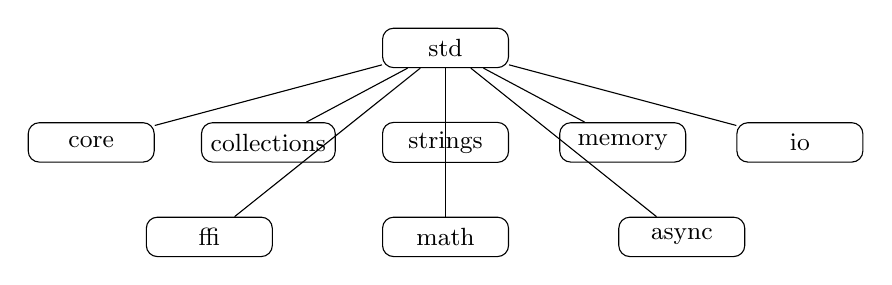
\begin{tikzpicture}[
    box/.style={rectangle, draw, rounded corners, minimum width=1.6cm, minimum height=0.5cm, font=\small}
]
    % Root node
    \node[box] (std) at (0,0) {std};

    % First row of children
    \node[box] (core) at (-4.5,-1.2) {core};
    \node[box] (collections) at (-2.25,-1.2) {collections};
    \node[box] (strings) at (0,-1.2) {strings};
    \node[box] (memory) at (2.25,-1.2) {memory};
    \node[box] (io) at (4.5,-1.2) {io};

    % Second row of children
    \node[box] (ffi) at (-3,-2.4) {ffi};
    \node[box] (math) at (0,-2.4) {math};
    \node[box] (async) at (3,-2.4) {async};

    % Draw connections
    \draw (std) -- (core);
    \draw (std) -- (collections);
    \draw (std) -- (strings);
    \draw (std) -- (memory);
    \draw (std) -- (io);
    \draw (std) -- (ffi);
    \draw (std) -- (math);
    \draw (std) -- (async);
\end{tikzpicture}
\end{center}

\subsection{Module Hierarchy}

\begin{description}
    \item[\texttt{std::core}] Fundamental types: \texttt{Option}, \texttt{Result}, core traits (\texttt{Drop}, \texttt{Clone}, \texttt{From})

    \item[\texttt{std::collections}] Data structures: \texttt{Vec}, \texttt{HashMap}, \texttt{HashSet}, \texttt{VecDeque}, \texttt{BitSet}, \texttt{SlotMap}

    \item[\texttt{std::string}] String handling: \texttt{Str} (borrowed), \texttt{String} (owned), \texttt{StringBuilder}, formatting

    \item[\texttt{std::memory}] Memory management: \texttt{MemoryBlock}, \texttt{Slice}, chip memory pools, allocators

    \item[\texttt{std::io}] Input/output: file operations, console I/O, ANSI terminal support

    \item[\texttt{amiga::raw}] AmigaOS bindings: Exec, DOS, Graphics, Intuition, and 70+ other libraries

    \item[\texttt{std::math}] Mathematics: fixed-point operations, vectors, angles, square roots

    \item[\texttt{std::async}] Asynchronous programming: futures, executors, sleep operations

    \item[\texttt{amiga::sys::hardware}] Hardware access: CPU detection, chipset identification, custom registers

    \item[\texttt{amiga::ui}] User interface: windows, screens, menus, gadgets, events

    \item[\texttt{amiga::sys::graphics}] Graphics operations: drawing, sprites, copper lists, blitter

    \item[\texttt{amiga::audio}] Audio playback: Paula channels, MOD players, sample management

    \item[\texttt{std::net}] Networking: TCP/UDP sockets, DNS, TLS (requires bsdsocket.library)

    \item[\texttt{std::test}] Testing framework: assertions, test attributes, benchmarking

    \item[\texttt{std::error}] Error types: \texttt{DosError}, \texttt{ExecError}, \texttt{NovusError}
\end{description}

\subsection{Physical Layout}

The library lives in the \texttt{std/} directory of the Novus installation:

\begin{lstlisting}[language=bash]
std/
    core.novus              # Core types (Option, Result, traits)
    prelude.novus           # Common re-exports
    collections/
        vec.novus           # Dynamic array
        hashmap.novus       # Hash map
        hashset.novus       # Hash set
        vecdeque.novus      # Double-ended queue
        bitset.novus        # Bit array
        slotmap.novus       # Generational arena
        ...
    strings/
        core.novus          # Str and String types
        format.novus        # Formatting utilities
        display.novus       # Display trait
    memory/
        block.novus         # MemoryBlock type
        slice.novus         # Slice operations
        chip.novus          # Chip memory utilities
        chip_pool.novus     # Chip memory pooling
        ...
    ffi/
        exec.novus          # Exec library
        dos.novus           # DOS library
        graphics.novus      # Graphics library
        intuition.novus     # Intuition library
        amiga_consts.novus  # All AmigaOS constants
        amiga_structs.novus # All AmigaOS structures
        ...
    ...
\end{lstlisting}

% ============================================================================
\section{The Prelude}
\label{sec:stdlib-prelude}
% ============================================================================

The prelude provides commonly-used types that you'll need in almost every program. Import it to get started quickly:

\begin{lstlisting}
from std::prelude import *
\end{lstlisting}

This imports:

\begin{itemize}
    \item \texttt{Option<T>} and \texttt{Result<T, E>} --- for safe error handling
    \item \texttt{Drop}, \texttt{From} --- core traits
    \item \texttt{Str} --- borrowed string type
    \item \texttt{DosError}, \texttt{ExecError}, \texttt{IntuitionError}, \texttt{GraphicsError}, \texttt{NovusError} --- error types
\end{itemize}

\subsection{Selective Imports}

For explicit control, import only what you need:

\begin{lstlisting}
from std::prelude import Option, Result
\end{lstlisting}

Or import directly from the source module:

\begin{lstlisting}
from std::core import Option, Result, Drop
from std::string import Str, String
from std::error::errors import DosError
\end{lstlisting}

\begin{comingfromc}
In C, you might include multiple headers to get the types you need:

\begin{lstlisting}[language=C]
#include <exec/types.h>
#include <dos/dos.h>
#include <string.h>
\end{lstlisting}

In Novus, the prelude gives you essentials in one import. For AmigaOS types, the \texttt{amiga::raw} modules are organized by library, not by NDK header structure.
\end{comingfromc}

% ============================================================================
\section{Import Conventions}
\label{sec:import-conventions}
% ============================================================================

Novus uses a consistent import ordering convention throughout the standard library and in idiomatic user code.

\subsection{Recommended Import Order}

\begin{lstlisting}
// 1. Core types first
from std::core import Option, Result, Drop, Clone

// 2. Collections
from std::collections::vec import Vec
from std::collections::hashmap import HashMap

// 3. Memory management
from std::memory::block import MemoryBlock
from std::memory::slice import Slice

// 4. Strings
from std::string import Str, String
from std::string import format

// 5. Error types
from std::error::errors import DosError, ExecError, NovusError

// 6. AmigaOS structures
from amiga::raw::structs import Window, Screen, RastPort

// 7. AmigaOS constants
from amiga::raw::consts import MEMF_PUBLIC, MEMF_CHIP

// 8. AmigaOS library functions
from amiga::raw::exec import AllocMem, FreeMem, Wait
from amiga::raw::dos import Open, Close, Read, Write
from amiga::raw::intuition import OpenWindow, CloseWindow

// 9. Other stdlib modules
from std::io::file import println
from std::math::vec2 import Vec2
\end{lstlisting}

\subsection{Wildcard Imports}

Use wildcard imports sparingly---they can cause name collisions:

\begin{lstlisting}
// OK: prelude is designed for wildcard import
from std::prelude import *

// OK: constants are namespaced and rarely collide
from amiga::raw::consts import *

// Avoid: too many names, potential collisions
from amiga::raw::exec import *
from amiga::raw::dos import *

// Better: import specific functions
from amiga::raw::exec import AllocMem, FreeMem, Wait
from amiga::raw::dos import Open, Close, Lock, UnLock
\end{lstlisting}

\subsection{Module Aliases}

For frequently-used modules with long paths, create local aliases:

\begin{lstlisting}
// Not yet supported - planned feature
// use amiga::raw::consts as consts
// use std::collections::hashmap as map

// Current workaround: import specific items
from amiga::raw::consts import MEMF_PUBLIC, MEMF_CHIP, MEMF_FAST
from amiga::raw::consts import MODE_OLDFILE, MODE_NEWFILE
\end{lstlisting}

% ============================================================================
\section{Core Types}
\label{sec:stdlib-core-types}
% ============================================================================

The \texttt{std::core} module defines the fundamental types that permeate all Novus code.

\subsection{Option<T>}

Represents a value that may or may not be present:

\begin{lstlisting}
pub enum Option<T> {
    Some(T),
    None,
}
\end{lstlisting}

\textbf{Key methods:}

\begin{center}
\begin{tabular}{lp{8cm}}
\textbf{Method} & \textbf{Description} \\
\hline
\texttt{is\_some()} & Returns \texttt{true} if value is present \\
\texttt{is\_none()} & Returns \texttt{true} if no value \\
\texttt{unwrap()} & Returns value, panics if \texttt{None} \\
\texttt{unwrap\_or(default)} & Returns value or default \\
\texttt{or(other)} & Returns self if \texttt{Some}, otherwise other \\
\texttt{FromPointer(ptr)} & Creates \texttt{Some} if non-null, \texttt{None} if null \\
\end{tabular}
\end{center}

\begin{lstlisting}
from std::core import Option

fn find_user(id: u32) -> Option<User> {
    if id == 0 {
        return Option::None
    }
    // ... lookup user ...
    return Option::Some(user)
}

// Usage
match find_user(42) {
    Option::Some(user) => println(user.name),
    Option::None => println("User not found")
}

// Or with unwrap_or
let user = find_user(42).unwrap_or(default_user)
\end{lstlisting}

\subsection{Result<T, E>}

Represents either success with a value or failure with an error:

\begin{lstlisting}
pub enum Result<T, E> {
    Ok(T),
    Err(E),
}
\end{lstlisting}

\textbf{Key methods:}

\begin{center}
\begin{tabular}{lp{8cm}}
\textbf{Method} & \textbf{Description} \\
\hline
\texttt{is\_ok()} & Returns \texttt{true} if success \\
\texttt{is\_err()} & Returns \texttt{true} if error \\
\texttt{unwrap()} & Returns value, panics if error \\
\texttt{unwrap\_or(default)} & Returns value or default \\
\texttt{ok()} & Converts to \texttt{Option<T>}, discarding error \\
\texttt{err()} & Converts to \texttt{Option<E>}, discarding value \\
\end{tabular}
\end{center}

\begin{lstlisting}
from std::core import Result
from std::error::errors import DosError

fn load_config(path: *u8) -> Result<Config, DosError> {
    let file = open(path, MODE_OLDFILE)?
    defer { close(file) }

    let data = read_all(&file)?
    parse_config(&data)
}

// Usage with ? operator
fn init() -> Result<(), DosError> {
    let config = load_config("app.cfg")?
    // ... use config ...
    Result::Ok(())
}

// Or with match
match load_config("app.cfg") {
    Result::Ok(config) => use_config(&config),
    Result::Err(e) => println(e.message())
}
\end{lstlisting}

\subsection{Core Traits}

\textbf{Drop} --- Automatic cleanup when a value goes out of scope:

\begin{lstlisting}
pub trait Drop {
    fn drop(&var self)
}

// Example: auto-closing file handle
impl Drop for FileHandle {
    fn drop(&var self) {
        if self.fh != null {
            unsafe { Close(self.fh) }
            self.fh = null
        }
    }
}
\end{lstlisting}

\textbf{Clone} --- Explicit value copying:

\begin{lstlisting}
pub trait Clone {
    fn clone(&self) -> Option<Self>
}

// Returns Option because cloning may allocate and fail
let original = Vec::new()
match original.clone() {
    Option::Some(copy) => { /* use copy */ },
    Option::None => { /* allocation failed */ }
}
\end{lstlisting}

\textbf{From} --- Type conversion:

\begin{lstlisting}
pub trait From<T> {
    fn convert(value: T) -> Self
}

// Example: DosError to NovusError
impl From<DosError> for NovusError {
    fn convert(e: DosError) -> NovusError {
        return NovusError::Dos(e)
    }
}

// Used automatically by ? operator
fn example() -> Result<(), NovusError> {
    let file = open("test.txt", MODE_OLDFILE)?  // DosError -> NovusError
    Result::Ok(())
}
\end{lstlisting}

% ============================================================================
\section{Error Types}
\label{sec:stdlib-errors}
% ============================================================================

The standard library provides error types for each AmigaOS subsystem.

\subsection{Error Type Hierarchy}

\begin{center}
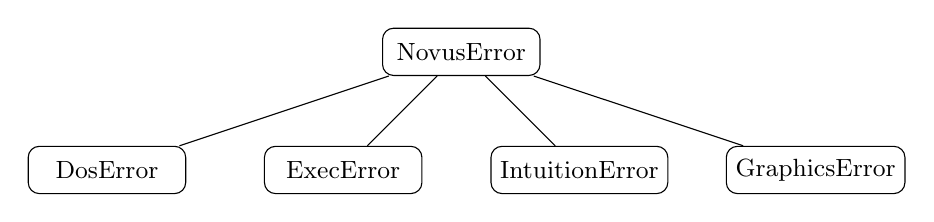
\begin{tikzpicture}[
    level 1/.style={sibling distance=3cm, level distance=1.5cm},
    every node/.style={rectangle, draw, rounded corners, minimum width=2cm, minimum height=0.6cm, font=\small}
]
    \node {NovusError}
        child { node {DosError} }
        child { node {ExecError} }
        child { node {IntuitionError} }
        child { node {GraphicsError} };
\end{tikzpicture}
\end{center}

\subsection{DosError}

Errors from the DOS library (most common variants shown):

\begin{lstlisting}
pub enum DosError {
    NotFound,           // Object not found (IoErr 205)
    AlreadyExists,      // Object already exists (IoErr 203)
    DirNotFound,        // Directory not found (IoErr 204)
    DirectoryNotEmpty,  // Can't delete non-empty dir (IoErr 216)
    PermissionDenied,   // Access denied
    WriteProtected,     // File write protected (IoErr 223)
    DiskFull,           // No space on disk (IoErr 221)
    NoDisk,             // No disk in drive (IoErr 226)
    InvalidLock,        // Bad file lock (IoErr 211)
    NoFreeStore,        // Out of memory (IoErr 103)
    ObjectInUse,        // Object is in use (IoErr 202)
    // ... plus 15+ more variants
    Unknown,            // Unmapped error code
}
\end{lstlisting}

\subsection{ExecError}

Errors from the Exec library:

\begin{lstlisting}
pub enum ExecError {
    NoMem,              // Memory allocation failed
    BadSignal,          // Invalid signal number
    NullReturn,         // Function returned NULL unexpectedly
    BadTask,            // Invalid task pointer
    BadNode,            // Invalid list node
    BadPort,            // Invalid message port
    SignalInUse,        // Signal already allocated
    TaskNotFound,       // FindTask failed
    LibraryNotFound,    // OpenLibrary failed
    InvalidAddress,     // Invalid memory address
    AlignmentError,     // Memory alignment violation
    IndexOutOfBounds,   // Array bounds violation
    CapacityExceeded,   // Fixed buffer full
}
\end{lstlisting}

\subsection{NovusError}

Wrapper for cross-subsystem error handling:

\begin{lstlisting}
pub enum NovusError {
    Dos(DosError),
    Exec(ExecError),
    Intuition(IntuitionError),
    Graphics(GraphicsError),
}

// All error types implement message()
impl DosError {
    pub fn message(&self) -> *u8 {
        match *self {
            DosError::NotFound => "Object not found",
            DosError::DiskFull => "Disk is full",
            // ...
        }
    }
}
\end{lstlisting}

\subsection{Converting Between Error Types}

The \texttt{?} operator automatically converts errors using the \texttt{From} trait:

\begin{lstlisting}
fn load_and_display(path: *u8) -> Result<(), NovusError> {
    // DosError automatically converts to NovusError
    let file = open(path, MODE_OLDFILE)?

    // ExecError also converts
    let buffer = MemoryBlock::alloc(1024, MEMF_PUBLIC)?

    Result::Ok(())
}
\end{lstlisting}

% ============================================================================
\section{Memory Allocation Conventions}
\label{sec:stdlib-memory}
% ============================================================================

The standard library follows consistent patterns for memory allocation.

\subsection{Fallible Allocation}

All allocating functions return \texttt{Option} or \texttt{Result}:

\begin{lstlisting}
// Vec allocation can fail - returns Result with error details
let vec = Vec::with_capacity(1000)?
// Or with explicit match:
match Vec::<i32>::with_capacity(1000) {
    Result::Ok(v) => { /* use v */ },
    Result::Err(e) => { /* out of memory: e.message() */ }
}

// MemoryBlock returns Option (simpler: worked or didn't)
match MemoryBlock::alloc(4096, MEMF_CHIP) {
    Option::Some(block) => { /* use block */ },
    Option::None => { /* allocation failed */ }
}
\end{lstlisting}

\subsection{Memory Type Flags}

AmigaOS memory flags are in \texttt{amiga::raw::amiga\_consts}:

\begin{lstlisting}
from amiga::raw::consts import MEMF_PUBLIC, MEMF_CHIP, MEMF_FAST
from amiga::raw::consts import MEMF_CLEAR, MEMF_LARGEST, MEMF_TOTAL

// Memory flags:
// MEMF_PUBLIC  - Accessible by other tasks
// MEMF_CHIP    - Chip RAM (DMA accessible)
// MEMF_FAST    - Fast RAM (CPU only)
// MEMF_CLEAR   - Zero-fill memory
// MEMF_LARGEST - Return largest available block
// MEMF_TOTAL   - Return total memory of type

// Typical patterns
let chip_buffer = MemoryBlock::alloc(size, MEMF_CHIP | MEMF_CLEAR)?
let fast_buffer = MemoryBlock::alloc(size, MEMF_FAST)?
let any_buffer = MemoryBlock::alloc(size, MEMF_PUBLIC)?
\end{lstlisting}

\subsection{RAII Memory Management}

All stdlib types that allocate implement \texttt{Drop}:

\begin{lstlisting}
fn process_data() -> Result<(), Error> {
    let vec = Vec::with_capacity(100).unwrap()
    let buffer = MemoryBlock::alloc(1024, MEMF_PUBLIC)?

    // ... use vec and buffer ...

    Result::Ok(())
}  // vec and buffer automatically freed here

// Even on early return:
fn early_exit() -> Result<(), Error> {
    let buffer = MemoryBlock::alloc(1024, MEMF_PUBLIC)?

    if some_condition {
        return Result::Err(Error::SomeError)  // buffer freed here
    }

    Result::Ok(())  // buffer freed here too
}
\end{lstlisting}

% ============================================================================
\section{AmigaOS FFI Organization}
\label{sec:stdlib-ffi}
% ============================================================================

The \texttt{amiga::raw} module provides bindings to AmigaOS libraries.

\subsection{Structure}

\begin{lstlisting}[language=bash]
std/amiga/raw/
    amiga_consts.novus    # ALL constants (combined)
    amiga_structs.novus   # ALL structures (combined)
    exec.novus            # Exec library functions
    dos.novus             # DOS library functions
    graphics.novus        # Graphics library functions
    intuition.novus       # Intuition library functions
    gadtools.novus        # GadTools library
    layers.novus          # Layers library
    utility.novus         # Utility library
    ... 70+ more libraries ...
\end{lstlisting}

\subsection{Using FFI Bindings}

\begin{lstlisting}
// Import structures
from amiga::raw::structs import Window, Screen, NewWindow

// Import constants
from amiga::raw::consts import WFLG_CLOSEGADGET, WFLG_DRAGBAR, WFLG_ACTIVATE
from amiga::raw::consts import IDCMP_CLOSEWINDOW, IDCMP_VANILLAKEY

// Import functions
from amiga::raw::intuition import OpenWindow, CloseWindow, WaitPort
from amiga::raw::exec import Wait

// Use in unsafe blocks
unsafe {
    let window = OpenWindow(&new_window_spec)
    if window != null {
        // ... use window ...
        CloseWindow(window)
    }
}
\end{lstlisting}

\subsection{Safe Wrappers}

Many FFI functions have safe wrappers in higher-level modules:

\begin{lstlisting}
// Low-level FFI (requires unsafe)
from amiga::raw::intuition import OpenWindowTags, CloseWindow

// High-level safe wrapper
from amiga::sys::intuition import WindowHandle, WindowBuilder

// Safe usage (no unsafe needed)
let window = WindowBuilder::new()
    .title("My Window")
    .size(320, 200)
    .close_gadget(true)
    .build()?

// Window automatically closed when dropped
\end{lstlisting}

\begin{comingfromc}
In C, you call AmigaOS functions directly and manage lifetimes manually:

\begin{lstlisting}[language=C]
struct Window *win = OpenWindowTags(NULL,
    WA_Title, "My Window",
    WA_Width, 320,
    WA_Height, 200,
    TAG_DONE);
// ... must remember to call CloseWindow(win) ...
\end{lstlisting}

In Novus, the safe wrappers handle cleanup automatically. You can still use the raw FFI when needed, but the wrappers are usually sufficient.
\end{comingfromc}

% ============================================================================
\section{Collections Overview}
\label{sec:stdlib-collections}
% ============================================================================

The \texttt{std::collections} module provides commonly-needed data structures.

\subsection{Available Collections}

\begin{center}
\begin{tabular}{llp{6cm}}
\textbf{Type} & \textbf{Module} & \textbf{Description} \\
\hline
\texttt{Vec<T>} & \texttt{vec} & Dynamic array, contiguous storage \\
\texttt{HashMap<K, V>} & \texttt{hashmap} & Key-value map with O(1) lookup \\
\texttt{HashSet<T>} & \texttt{hashset} & Unique values with O(1) contains \\
\texttt{VecDeque<T>} & \texttt{vecdeque} & Double-ended queue \\
\texttt{BitSet} & \texttt{bitset} & Compact bit array \\
\texttt{SlotMap<T>} & \texttt{slotmap} & Generational arena with stable keys \\
\texttt{RingBuffer<T>} & \texttt{ringbuffer} & Fixed-size circular buffer \\
\texttt{FreeList<T>} & \texttt{freelist} & Object pool with recycling \\
\texttt{SmallVec<T, N>} & \texttt{smallvec} & Stack-allocated up to N elements \\
\texttt{IntrusiveList<T>} & \texttt{intrusive\_list} & Linked list with embedded nodes \\
\end{tabular}
\end{center}

\subsection{Common Patterns}

\begin{lstlisting}
from std::collections::vec import Vec
from std::collections::hashmap import HashMap

// Dynamic array
var scores: Vec<i32> = Vec::new()
scores.push(100)?
scores.push(85)?
scores.push(92)?

for i in 0..scores.len() {
    let score = scores.get(i).unwrap()
    println(f"Score: {score}")
}

// Hash map
var names = HashMap::<u32, *u8>::new()?
names.insert(1, "Alice")?
names.insert(2, "Bob")?

match names.get(1) {
    Option::Some(name) => println(name),
    Option::None => println("Not found")
}
\end{lstlisting}

% ============================================================================
\section{Strings Overview}
\label{sec:stdlib-strings}
% ============================================================================

Novus provides two main string types for different use cases.

\subsection{String Types}

\begin{center}
\begin{tabular}{llp{6cm}}
\textbf{Type} & \textbf{Ownership} & \textbf{Use Case} \\
\hline
\texttt{*u8} & Borrowed & Literal strings, C interop \\
\texttt{Str} & Borrowed & String views with length \\
\texttt{String} & Owned & Mutable, growable strings \\
\texttt{StringBuilder} & Owned & Efficient string building \\
\end{tabular}
\end{center}

\subsection{Usage Examples}

\begin{lstlisting}
from std::string import Str, String, StringBuilder

// Literal (null-terminated, borrowed)
let greeting: *u8 = "Hello, Amiga!"

// Str - borrowed view with known length
let s = Str::from_cstr("Hello").unwrap()
println(f"Length: {s.len()}")

// String - owned, mutable
var name = String::from("Hello")
name.push_str(", World!")
println(name.as_cstr())

// StringBuilder - efficient concatenation
var builder = StringBuilder::new()
builder.push_str("Line 1\n")
builder.push_str("Line 2\n")
builder.push_str("Line 3\n")
let result = builder.to_string()
\end{lstlisting}

% ============================================================================
\section{I/O Overview}
\label{sec:stdlib-io}
% ============================================================================

The \texttt{std::io} module handles input and output operations.

\subsection{Console Output}

\begin{lstlisting}
from std::io::file import print, println

// Basic output
println("Hello, World!")

// With formatting (f-strings)
let name = "Amiga"
let year = 1985
println(f"The {name} was released in {year}")

// Without newline
print("Enter name: ")
\end{lstlisting}

\subsection{File Operations}

\begin{lstlisting}
from amiga::sys::dos import open, close, read, write
from amiga::raw::consts import MODE_OLDFILE, MODE_NEWFILE

// Reading a file
fn read_file(path: *u8) -> Result<Vec<u8>, DosError> {
    let file = open(path, MODE_OLDFILE)?
    defer { close(file) }

    var buffer: Vec<u8> = Vec::with_capacity(4096).unwrap()
    // ... read into buffer ...
    Result::Ok(buffer)
}

// Writing a file
fn write_file(path: *u8, data: &[u8]) -> Result<(), DosError> {
    let file = open(path, MODE_NEWFILE)?
    defer { close(file) }

    write(&file, data)?
    Result::Ok(())
}
\end{lstlisting}

% ============================================================================
\section{Design Principles}
\label{sec:stdlib-principles}
% ============================================================================

The standard library follows several guiding principles.

\subsection{Amiga First}

The library is designed specifically for AmigaOS, not as a portable abstraction layer:

\begin{itemize}
    \item Memory types (chip/fast) are first-class concepts
    \item AmigaOS error codes map directly to error types
    \item Custom chip access is supported, not hidden
    \item RAII works with AmigaOS resource management patterns
\end{itemize}

\subsection{Zero-Cost Abstractions}

High-level types compile to efficient code:

\begin{lstlisting}
// Vec<i32> with bounds checking
let value = vec.get(index)?

// In release mode, compiles to roughly:
//   move.l (a0,d0.l*4),d0
// The Option wrapper is optimized away
\end{lstlisting}

\subsection{Explicit Allocation}

Every allocation is visible and can fail:

\begin{lstlisting}
// Allocations return Option or Result
let vec = Vec::with_capacity(1000)?  // Returns Result<Vec, ExecError>
let map = HashMap::new()?            // Returns Result<HashMap, ExecError>
map.insert(key, value)?              // Allocation happens here
\end{lstlisting}

\subsection{Safe Defaults, Unsafe Escape Hatch}

Most code uses safe wrappers. Raw FFI is available when needed:

\begin{lstlisting}
// Safe (preferred)
let window = Window::open(&spec)?

// Unsafe (when needed)
unsafe {
    let raw_window = OpenWindow(&raw_spec)
}
\end{lstlisting}

% ============================================================================
\section{What's Covered in Part II}
\label{sec:stdlib-roadmap}
% ============================================================================

The following chapters cover each module area in depth:

\begin{description}
    \item[Chapter 13: Core Types] Complete coverage of \texttt{Option}, \texttt{Result}, and core traits

    \item[Chapter 14: Collections] All collection types with performance characteristics and usage patterns

    \item[Chapter 15: Strings] String types, formatting, parsing, and Unicode handling

    \item[Chapter 16: Memory] Memory management, allocators, pools, and chip memory handling

    \item[Chapter 17: I/O] File operations, console I/O, formatting, and buffering

    \item[Chapter 18: Math] Fixed-point arithmetic, vectors, matrices, and trigonometry

    \item[Chapter 19: AmigaOS Bindings] Using the FFI layer, calling conventions, and safe wrappers
\end{description}

% ============================================================================
\section{Quick Reference}
\label{sec:stdlib-quick-ref}
% ============================================================================

\subsection{Common Imports}

\begin{lstlisting}
// Everything you need for most programs
from std::prelude import *
from std::collections::vec import Vec
from std::io::file import println
from amiga::raw::consts import MEMF_PUBLIC, MEMF_CHIP
\end{lstlisting}

\subsection{Error Handling Pattern}

\begin{lstlisting}
fn main() -> i32 {
    match run() {
        Result::Ok(_) => return 0,
        Result::Err(e) => {
            println(e.message())
            return 1
        }
    }
}

fn run() -> Result<(), NovusError> {
    let config = load_config()?
    let window = open_window(&config)?
    main_loop(&window)?
    Result::Ok(())
}
\end{lstlisting}

\subsection{Memory Allocation Pattern}

\begin{lstlisting}
fn process() -> Result<(), ExecError> {
    // Allocation returns Result
    let buffer = MemoryBlock::alloc(4096, MEMF_PUBLIC)?
    defer { /* buffer automatically freed */ }

    // Use buffer...
    do_work(buffer.as_slice())

    Result::Ok(())
}
\end{lstlisting}

% ============================================================================
\section{Summary}
\label{sec:stdlib-summary}
% ============================================================================

The Novus standard library provides:

\begin{itemize}
    \item \textbf{Core types} --- \texttt{Option}, \texttt{Result}, and traits for safe error handling
    \item \textbf{Collections} --- \texttt{Vec}, \texttt{HashMap}, and specialized containers
    \item \textbf{Strings} --- Borrowed and owned strings with formatting
    \item \textbf{Memory} --- Safe allocation with RAII cleanup
    \item \textbf{I/O} --- File and console operations
    \item \textbf{FFI} --- Complete AmigaOS library bindings
    \item \textbf{Math} --- Fixed-point arithmetic and vectors
    \item \textbf{Async} --- Cooperative multitasking via Exec signals
\end{itemize}

The library is designed for the Amiga: every feature respects the platform's constraints while providing modern ergonomics. Use the prelude for quick starts, import specific modules for explicit control.

The following chapters explore each module in depth, with complete API references and practical examples.
